\documentclass[a4paper]{article}

\usepackage{conference}
\usepackage{times}

\usepackage{graphicx}
\usepackage{epstopdf}

\usepackage{caption}
\usepackage{subcaption}

\usepackage{amsmath}
\usepackage{amssymb}

\usepackage{url}

\usepackage{color}
\newcommand{\todo}[1]{{\small\color{red}[#1]}}


\title{Collaboration in Ad Hoc Teamwork: \\
Ambiguous Tasks, Roles, and Communication\vspace{1em}}

% \author{Anonymous authors for blind review}
\setlength\titlebox{3.8in}

\author{
Jonathan Grizou \\ Flowers Team \\ INRIA - ENSTA ParisTech \\  France \\ jonathan.grizou@inria.fr
\And
Samuel Barrett \\ Kiva Systems \\ North Reading, MA 01864 USA \\ basamuel@kivasystems.com
\AND
Peter Stone \\ Dept. of Computer Science \\ The Univ. of Texas at Austin \\ Austin, TX 78712 USA \\ pstone@cs.utexas.edu
\And
Manuel Lopes \\ Flowers Team \\ INRIA - ENSTA ParisTech \\  France \\ manuel.lopes@inria.fr
}

\newcommand{\env}{E}
\newcommand{\task}{\tau}
\newcommand{\conf}{\kappa}
\newcommand{\com}{\rho}
\newcommand{\gridwidth}{1}
\newcommand{\figwidth}{1}

\DeclareMathOperator*{\argmax}{\arg\!\max}

%CHEAT CODES
% \renewcommand{\baselinestretch}{.98}

\begin{document}

\maketitle

\begin{abstract}
Autonomous agents are becoming increasingly present in our environments, and will increasingly have to collaborate with previously unseen agents. Creating autonomous agents capable of cooperating with previously unfamiliar teammates, known as ``ad hoc teamwork'', has been identified as an important challenge for multiagent systems. Previous research has assumed that either the task, the role of each agent, or the communication protocol among agents is known before the interaction begins. In this paper, we consider these three variables simultaneously and show how an ad hoc agent can fit into a new team while handling ambiguous tasks, roles, and communication protocols. We assume a known distribution of possible tasks, roles, and communication protocols. We present experimental results in the pursuit domain showing that an ad hoc agent can integrate itself into a team by quickly identifying the task, selecting its role on the team, and estimating the communication protocol being used; thus barely impacting the overall team performance compared to a pre-coordinated agent.
\end{abstract}

\section{Introduction}

% As robots are moving into the real world, they will need to engage in cooperative activities with previously unknown teammates.

There are many situations where an international effort is needed to address a particular well focused problem, e.g. rescue efforts in a natural disaster area. In this setting, multiple robots might be available, but they do not have the same software and hardware, and they will not communicate and coordinate using standard protocols. Nevertheless, they should coordinate to achieve a common goal, even if team coordination strategies cannot be pre-defined.

This challenge of multi-agent interaction without pre-coordination is also called the pickup team challenge \cite{gil2006dynamically} or the ad hoc team challenge \cite{stone2010ad}. It states that agents should learn to collaborate without defining pre-coordination schemes and/or without knowing what the other agents are capable of \cite{bowling2005coordination,gil2006dynamically,stone2010ad}.

In this work, we focus on the ad hoc team challenge (\cite{stone2010ad}). We imagine a team of specialized agents that work to achieve a specific task and coordinate using a specific language. We introduce a new algorithm allowing an ad hoc agent to join and collaborate with such a team. The ad hoc agent must take its role in the team and must therefore identify the three following components:
%
\begin{itemize}
\item the \textbf{task} the team is trying to solve, so as to help the team achieve it;
\item the \textbf{role} of each agent, so as to replace the missing specialized agent;
\item the \textbf{communication protocol} used by the team, so as to be informed of important facts concerning the task.
\end{itemize}
%
We present empirical results in the pursuit domain showing that an ad hoc agent can efficiently replace any member of such a team. For this purpose, we assume the ad hoc agent has access to a set of hypotheses about the possible tasks, team configurations, and communication systems. Given this information it is possible to infer which hypothesis is the most likely given the observations of other agents' movements and communications. We show that the default team performance is quickly recovered after our ad hoc agent is included and further show that our algorithm is robust to noise.

%In the following sections, we formally define the problem and describe how an ad hoc agent can infer which hypothesis is correct one select its actions. We then describe the pursuit domain used for testing our algorithm, as well as the possible tasks, team configurations, and communication systems. In Section \ref{sec:results}, we compare the default team performance with the one including the ad hoc agent. Finally, we propose a number of directions for future work and highlight related work from other fields of research.

\section{Related Work}

Previous research focused on different variations of the problem.

\textbf{How an ad hoc agent can influence its teammates to achieve a new task} (\cite{stone2013teaching}). It is usually assumed that teammates have limited action capabilities and a fixed and known behavior. Furthermore, only the ad hoc agent is aware of the goal of the task and has to influence the behaviors of the others to fulfill it. \cite{stone2010teach,stone2013teaching} define the general problem and provide a solution for the two agents scenario. Extension to the multi-teammates case is presented by \cite{agmon12leading}. An interesting application is the study of how an ad hoc agent can learn to lead a flock of agents (\cite{genter2013flock}).
% Such work assumes prior knowledge of a generative model of the teammate’s policy that generates sample trajectories of their behavior.

\textbf{How an ad hoc agent can adapt in a pre-formed team, with the specific aim of optimally helping the team to achieve its goal} (\cite{barrett2013team}). It is usually assumed the task to achieve is known to the ad hoc agent. In a first approach the model of the other agents was known \cite{barrett2011empirical}, but this assumption was progressively removed: first, by assuming agents were drawn from a set of possible agents \cite{barrett2011empirical,genter2011role}, and then, by learning online a model of each teammate \cite{barrett2013team} -- even considering learning abilities from the other agents \cite{chakraborty2013cooperating}.

\textbf{How an ad hoc agent can best communicate with its teammates} (\cite{barrett2014communicating}). This recent work assumes the ad hoc agent is omniscient -- knowing the task, the model of the agents, and the communication protocol. However, the ad hoc agent does not always knows how its teammates would react to its messages. The problem was how to optimally communicate with other agents to improve the team performance in a k-armed bandit problem.

This paper differs from previous work in that the ad hoc agent is not informed of the task to be achieved and does not initially understand the communication of the other agents. This work shares similarities with previous work in that our team includes specialized agents, as in \cite{genter2011role}, and we will assume a finite set of possible teammates and domain configurations, as in \cite{genter2011role,barrett2011empirical,barrett2014communicating}.

% \todo{Confusing sentence:::: Contrary to previous approaches, the ad hoc agent will simply try to fulfill the role of the missing agent, but previous studies already demonstrated that a team-aware ad hoc agent could even improve the default team performance \cite{barrett2011empirical,chakraborty2013cooperating}.}

A similar problem, where both the task and the communication are unknown, has already been investigated in human-machine interaction \cite{grizou2014interactive}. They consider only two agents, a teacher and a learner. The learning agent has access to even less information than the scenario presented here -- it could not observe the actions of the other agent and could only act on its own towards the success of the task. However, the learner could observe non-symbolic communication signals from the other agent, whose meaning, i.e. its language, was initially unknown. Bringing their work to the multi-agent problem is not straightforward and would require additional developments not considered in this work.

% A similar problem, where both the task and the communication are unknown, has already been investigated in human-machine interaction \cite{grizou2013robot,grizou2014interactive}. In their work, the learning agent has access to even less information than the scenario presented here -- it could not observe the actions of the other agent and could only act on its own towards the success of the task. However the learner could observe non-symbolic communication signals from the other agent, whose meaning, i.e. its language, was initially unknown. It lead to interesting application for calibration-free brain-computer interaction \cite{grizou2014calibration}. They propose ways to extend their approach to continuous state space and an infinite set of task, but bringing their work to the multi-agent problem is not straightforward and would require additional developments not considered in this work.

% Our aim with the paper is to show that these unknowns, which are usually considered separately, can be considered jointly. To this end we designed a default team that is fully functional. This team has to achieve a given task, each agent in the team has a specific role, and they all communicate given a specific protocol. The aim of our experiment is to study how an ad hoc agent can fit and collaborate with such a team. To this end, we randomly remove an agent from a working team and insert our ad hoc agent. The ad hoc agent must take the role of the missing agent and must therefore infer what is the task, the team configuration, and the communication protocol.

% Indeed, it is difficult to infer the communication if we do not know the task, or to infer the task if we do not know the role of each agent. Yet, it is unlikely that all agents in a team share any of the above-mentioned information before practical interaction.

% We identified three usual sources of uncertainty an ad hoc agent faces in most scenarios: the task, the team configuration, and the communication protocol.


\section{Fluid Collaboration in Ad Hoc Teamwork}
\label{sec:problem}

\subsection{Problem Definition}

We consider a team $B$ of $n_B$ agents $B = \{b_1, \ldots , b_{n_B}\}$ that is functional and well suited to solve the task from a domain $d \in D$. A domain is made of four components:

\begin{itemize}
\item An \textbf{environment} $\env$ made of $n_S$ states, which we denote $\{s_1, \ldots, s_{n_S}\}$, and where agents can perform $n_U$ actions, which we denote $\{u_1, \ldots, u_{n_U}\}$. The environment dynamics are known and described by a probability distribution that for any given state $s$ and action $u$ gives the probability of a next state $s'$, $p(s'|s,u,\env)$.
\item A \textbf{task} $\task$ that the agents should achieve, represented by a reward function $R$.
\item A \textbf{configuration} $\conf$ that defines the role given to each agent, i.e. their specialties.
\item A \textbf{protocol} $\com$ that defines the way agents communicate to each others, i.e. their language. We denote $m_{b}$ as the message of an agent $b$.
\end{itemize}

A domain is defined by $d = \{\env, \task, \conf, \com\}$ that is a subset of all possible domains $D$. We denote $S$ as the set of all agent states, $ S~=~\{ s_{b_1}, \ldots, s_{b_{n_B}} \} $, respectively $S'$ the set of all agent next states. We denote $M$ as the set of all agents' messages, $M~=~\{m_{b_1}, \ldots, m_{b_{n_B}}\}$. We want to evaluate how an ad hoc agent $a$ can adapt in such a domain. To evaluate its performance, we remove one agent randomly from a fully formed team, creating the set $B^-$, and replace it by the ad hoc agent. The resulting team is denoted as $B^{-}_{a}$.
%
The team performance is evaluated on the task $\task$ using the reward function $R$. We denote $score(B, d)$ as the score resulting from the team $B$ executing the problem $d$, i.e. the accumulated reward. In this work, we want to create an ad hoc agent that minimizes the score loss between the original team $score(B, d)$ and the team with the ad hoc agent $score(B^{-}_{a}, d)$. The problem is that the ad hoc agent needs to fit into a team yet unknown to it. It must therefore identify all the components of the domain ($\env, \task, \conf, \com$). The main challenge is that the ad hoc agent does not have direct access to its performance. Indeed, it cannot compute $score(B^{-}_{a}, d)$ because $d$ is unknown to it.

\subsection{Algorithm}

To tackle this problem, we assume the agent has access to a bigger set $D = \{d_1, \ldots, d_{n_H}\}$, containing $n_H$ possible domains, from which is pulled the particular domain $d$ considered. We further consider that, for any given $d_h$, the ad hoc agent can predict, in a probabilistic way, the expected behavior and communication of the agents. Hence, our approach relies on computing the posterior probability of each hypothetical domain given the information available to the ad hoc agent, here the observation from states and messages of the other agents. The correct hypothesis will be the one that maximizes this probability:
%
\begin{eqnarray}
\argmax_h~~p(d_h|S',S,M)  \label{eq:problem}
\end{eqnarray}
%
where $S$ and $S'$ are the observed states and next states, and $M$ is the messages sent by each agent. At each step a new tuple $\{S', S, M\}$ is observed and the probabilities are updated. Following Bayes' rule, we have to compute two different components: first the probability of the observed next states given the initial states, the messages, and a domain hypothesis $p(S'|S,M,d_h)$, and then the probability of the messages themselves given the oberved states and a domain hypothesis $p(M|S,d_h)$. In the following subsections, we detail these components as well as how the ad hoc agent plans its actions.% first how to use observations of the state of other agents, then how to exploit their messages, and finally

\subsubsection{Using state observations}

Observing the behavior of all other agents is a valuable source of information. Given a hypothesis domain $d_h$, we can compute the probability of the next agent state $S'$ given the current agent state $S$. For each hypothesis, we create a Bayes' filter that accumulates the probability of each domain conditionally on the observation of the agent movements.
To do so, we must estimate the probability that each agent selected each available action. We then estimate the probability of the observed state given all possible combinations of agents' actions and the environment dynamics:
% We denote that the computational cost of such update rule rises quickly with the number of agents.
%
\begin{eqnarray}
p(d_h|S',S) &\propto& p(S'|S,d_h) p(d_h)
\label{eq:obsupdate}
\end{eqnarray}
%
with
%
\begin{eqnarray}
p(S'|S,d_h) = \prod_i \sum_j p(s'_{b_i}|s_{b_i},u_j,\env_h) p(u_j|s_{b_i}, S, d_h)
\label{eq:obsupdateexpanded}
\end{eqnarray}
%
where $\env_h$ is the environment in $d_h$ which includes the state transition model. And $p(u_j|s_{b_i}, S, d_h)$ is the model of agent $b_i$ action selection, which is based on all the components of $d_h$ and the current state of the domain $S$. Given the agents' roles, their actions are independent. % But this might not always be the case, as exemplified in the pursuit domain example of section~\ref{sec:domain}. To accommodate with this

The equation above considers the case of full observability of the states. As this might not always be true (e.g. partial observability from the ad hoc agent in section~\ref{sec:com}), the update rule should also account for partial observability, represented by a discrete probabily distribution on $S$ and $S'$. The update becomes:
%
\begin{eqnarray}
p(d_h) &=& \sum_{S'} \sum_S p(d_h|S',S) p(S') p(S)
\label{eq:obsupdatestateprob}
\end{eqnarray}
%
which can be expanded as Equation~\ref{eq:obsupdate} is in Equation~\ref{eq:obsupdateexpanded}.

\subsubsection{Using communication}

Communication can greatly benefit coordination in a team. In our setting, the messages exchanged can provide two valuable types of information. First, in case of partial state observation, they help narrow the probability of the states:
%
\begin{eqnarray}
p(S|M, S^{obs}, d_h)
\label{eq:stateupdate}
\end{eqnarray}
%
with $S^{obs}$ being the state observed by the agent. This is helpful to narrow down the update in equation~\ref{eq:obsupdatestateprob}. Second, given a specific domain hypothesis $d_h$, they can be used to test the coherence of the messages agents sent based on the associated communication protocol $\com_h$. For example, if messages from all agents do not indicate concordant information, and if they cannot be explained by communication noise, then the communication protocol associated to the domain hypothesis $d_h$ is not the one used by the team. This results in an additional domain probability update rule:
%
\begin{eqnarray}
p(d_h|M,S) &\propto& p(M|S,d_h) p(d_h)
\label{eq:messageupdate}
\end{eqnarray}
%
The set of equations defined above are generic update rules for an ad hoc agent to infer which domain it is facing. Details about their particular implementation for the pursuit domain are provided in the following sections.

\subsubsection{Planning}

We now consider the action selection method for the ad hoc agent. Previous work considered ad hoc agents that solve the optimal teammate problem. Such agents know the model of their teammates and select their next action in order to improve maximally the team performance -- often resulting in better performance than the initial team \cite{barrett2011empirical}. The aim of this study is different; we want to advocate the fact that the ad hoc agent can work under less assumptions than before and be able to estimate more information about the new team. Hence, we isolate our algorithm from the planning aspects and test whether it can select between candidate domains. Therefore, in this work, the ad hoc agent simply tries to replace a missing agent in the team. To this end, the ad hoc agent will weight the policies for each domain hypotheses $d_h$ by the probability currently assigned to this configuration $p(d_h)$.
%
\begin{eqnarray}
p(u_a|M, S) = \sum_h p(u_a|M, S, d_h) p(d_h)
\label{eq:adhocpolicy}
\end{eqnarray}
%
With this planning strategy, once the correct hypothesis is identified, the ad hoc agent will mimic the default behavior of the agent it replaces. But the agent is likely to make sensible decision earlier as irrelevant hypotheses are discarded.

% Nothing limits us to the use of this policy and more advanced planning strategies -- which have already been shown to be beneficial in this kind of scenario \cite{barrett2011empirical} -- could be considered.


\section{Pursuit Domain}
\label{sec:domain}

\begin{figure*}[t]
\centering
\begin{subfigure}[t]{0.19\textwidth}
\centering
\captionsetup{width=0.9\textwidth}
\includegraphics[trim=7cm 3cm 6cm 2cm, clip=true, width=\gridwidth\textwidth]{plots/visuals/teamConfigRandom.png}
\caption{A random position.}
\label{fig:randpos}
\end{subfigure}
\begin{subfigure}[t]{0.19\textwidth}
\centering
\captionsetup{width=0.9\textwidth}
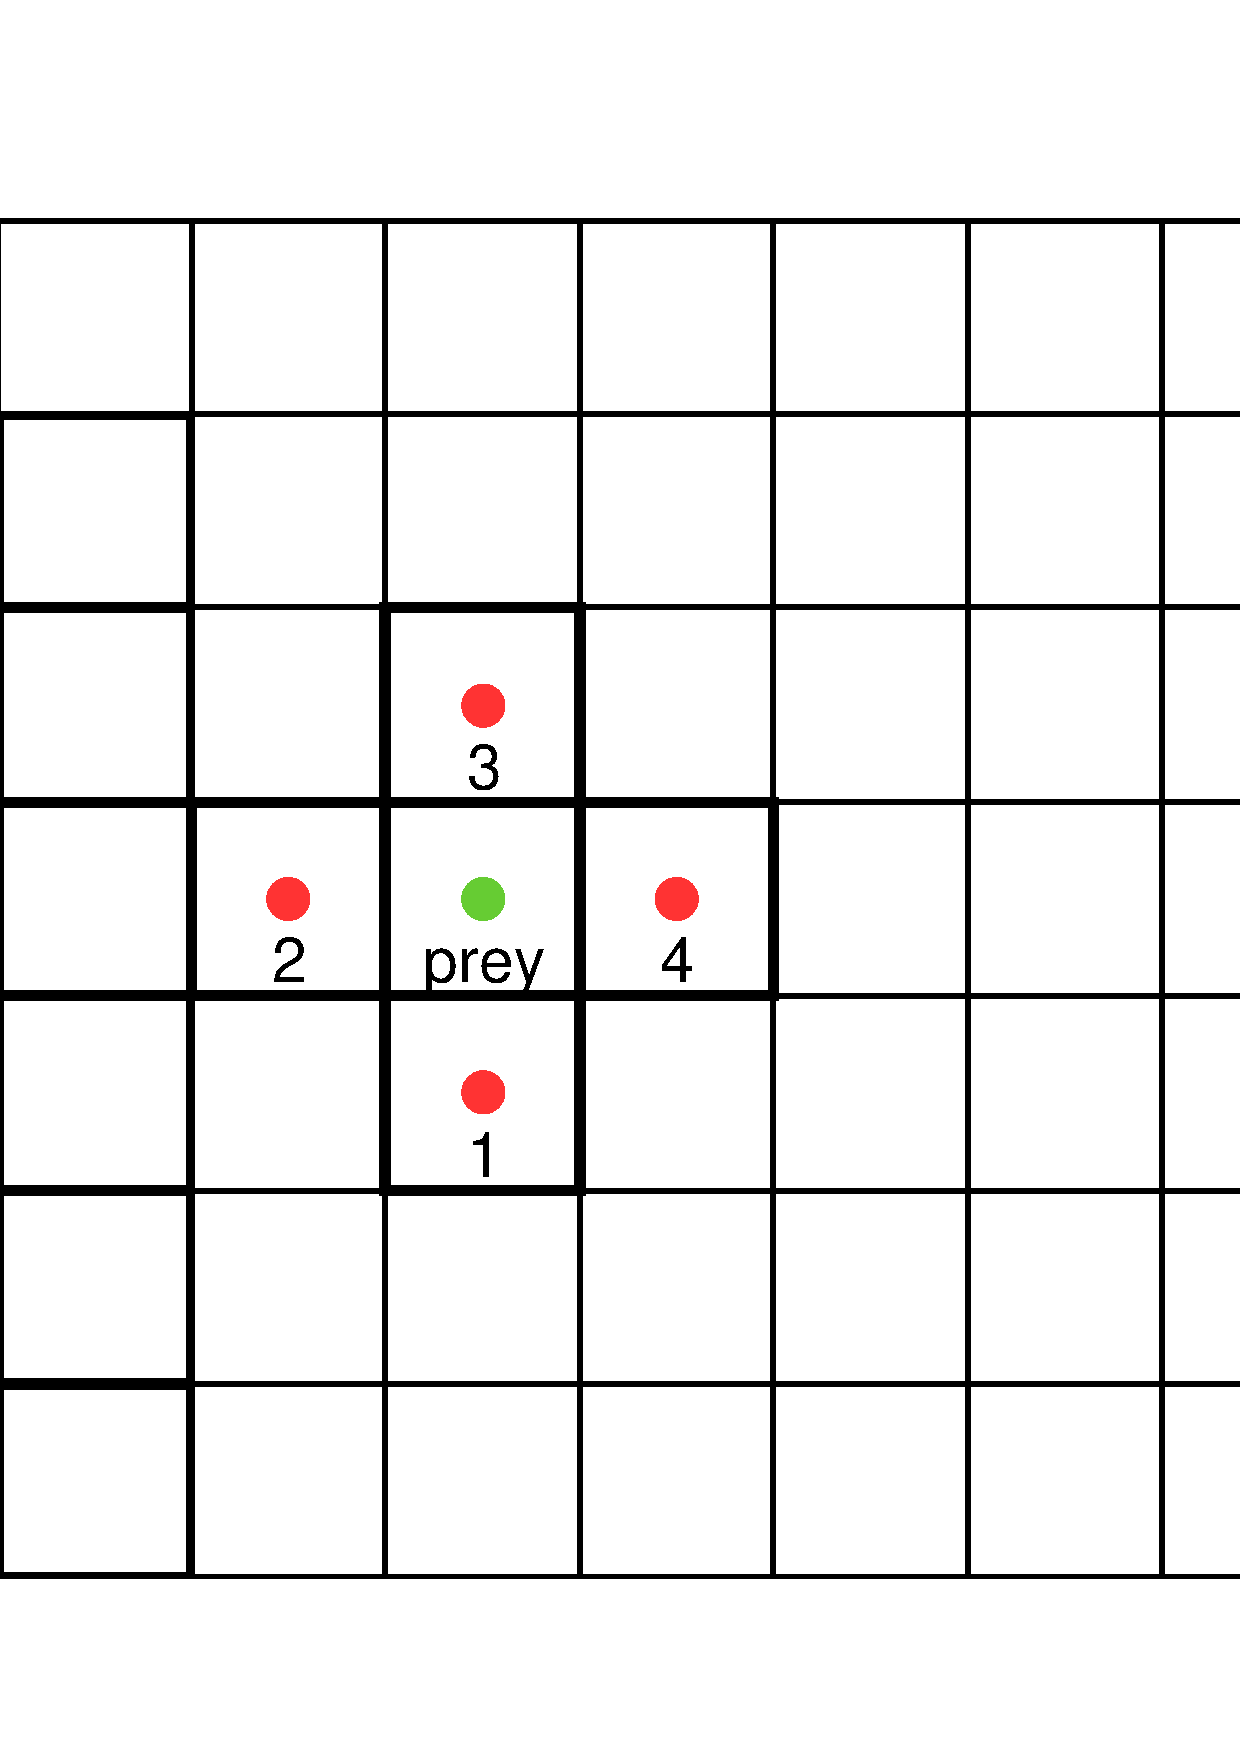
\includegraphics[trim=7cm 3cm 6cm 2cm, clip=true, width=\gridwidth\textwidth]{plots/visuals/teamConfigCapture.png}
\caption{A capture position.}    \label{fig:capturepos}
\end{subfigure}
\begin{subfigure}[t]{0.19\textwidth}
\centering
\captionsetup{width=0.9\textwidth}
\includegraphics[trim=7cm 3cm 6cm 2cm, clip=true, width=\gridwidth\textwidth]{plots/visuals/teamConfigApproach.png}
\caption{The predators chasing the prey to the North-East.}
\label{fig:capturepos}
\end{subfigure}
\begin{subfigure}[t]{0.19\textwidth}
\centering
\captionsetup{width=0.9\textwidth}
\includegraphics[trim=7cm 3cm 6cm 2cm, clip=true, width=\gridwidth\textwidth]{plots/visuals/targetStates_11.png}
\caption{States to target for each predator, chasing East.}
\label{fig:role11}
\end{subfigure}
\begin{subfigure}[t]{0.19\textwidth}
\centering
\captionsetup{width=0.9\textwidth}
\includegraphics[trim=7cm 3cm 6cm 2cm, clip=true, width=\gridwidth\textwidth]{plots/visuals/visibleStatesMiddle.png}
\caption{States observable by a predator in position (3,3).}
\label{fig:visiblecenter}
\end{subfigure}
\caption{Illustration of the pursuit domain, the team strategy, and the partial observability. The green circle is the prey and the red ones are predators. The cell with a blue circle marked with \small{\emph{CS}} is the capture state.\vspace{-0.3cm}}
\label{fig:illustration}
\end{figure*}

We test our approach in a variant of the pursuit domain \cite{benda1986empirical}. The pursuit domain is often used in the multi-agent literature \cite{stone2000multiagent} including in ad hoc team scenarios \cite{barrett2011empirical} and involves a set of predators aiming at capturing a prey. We consider a 2D discrete toroidal 7x7 grid world (an agent leaving from one side of the grid will ``reappear'' on the opposite side), 4 predators, and 1 prey. Agents can perform 5 actions: North, South, East, West, and a ``no move'' action. The task is to lock the prey on a particular grid cell, called the capture state. To capture the prey, the predators must encircle it (i.e. one predator on each grid cell nearby the prey). This problem is well-suited for the ad hoc challenge because the task cannot be performed by a subset of the predators alone -- all team members play a key role in accomplishing the task. Figure~\ref{fig:randpos} and \ref{fig:capturepos} illustrate a random team state and a capture position. For the teams used in this work, each predator is allocated a specific role in the team, i.e. taking one side of the prey (North, South, East, or West). In an advanced scenario, the predators have only partial observability, which dramatically decreases team efficiency. To overcome this problem, the predators are given the ability to communicate -- using a specific protocol -- about the prey position. Finally, noise is added to actions and communications.


% \begin{figure}%   \centering%   \begin{subfigure}[b]{0.49\columnwidth}%     \centering%     \includegraphics[trim=7cm 3cm 6cm 2cm, clip=true, width=\gridwidth\columnwidth]{plots/visuals/teamConfigRandom.png}%     \caption{A random position}%     \label{subfig:randpos}%   \end{subfigure}%   \begin{subfigure}[b]{0.49\columnwidth}%     \centering%     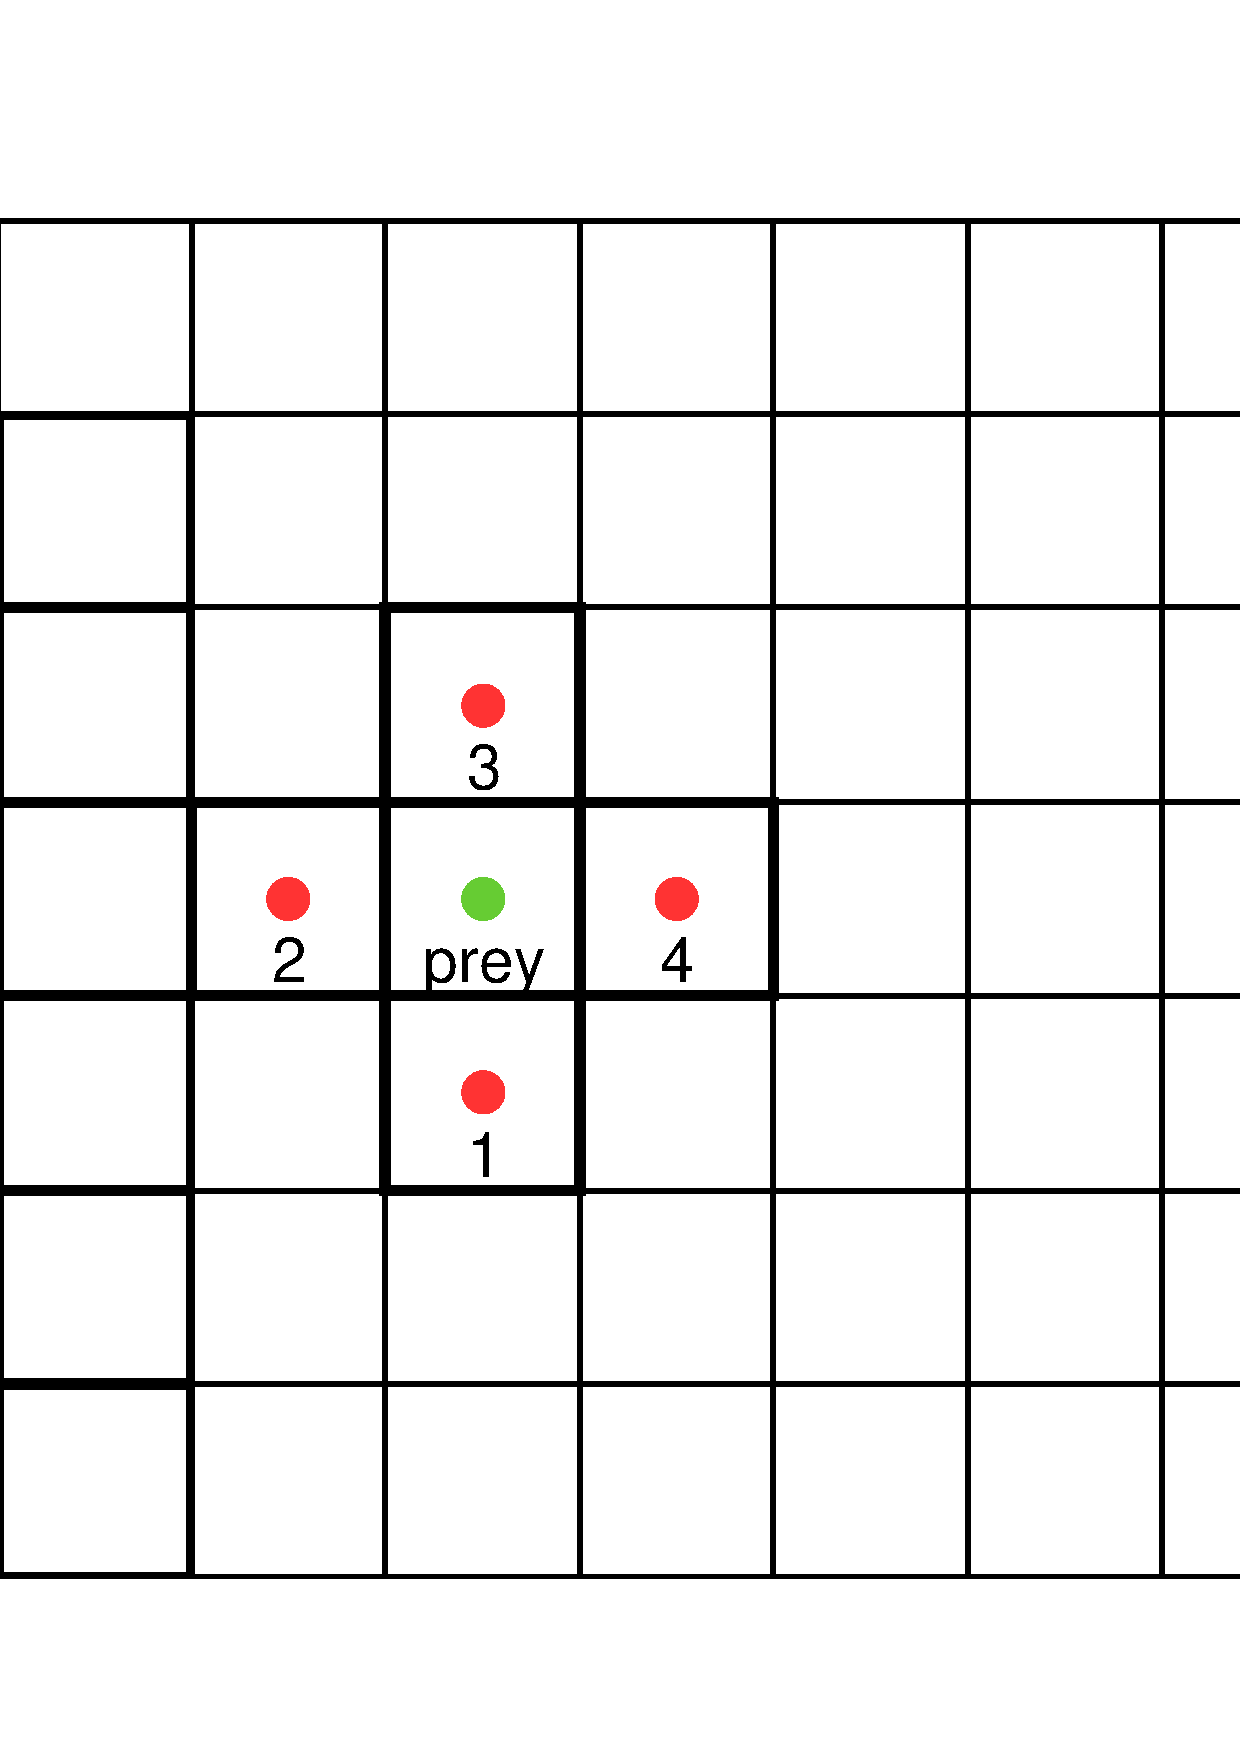
\includegraphics[trim=7cm 3cm 6cm 2cm, clip=true, width=\gridwidth\columnwidth]{plots/visuals/teamConfigCapture.png}%     \caption{A capture position}%     \label{subfig:capturepos}%   \end{subfigure}%   \caption{Start and capture position in the pursuit domain. The green circle is the prey and the red ones are predators. The cell with a blue circle marked with \emph{CS} is the capture state.}%   \label{fig:samplepos}% \end{figure}

In the remainder of this section, we describe how agents plan their actions, as well as the strategy of the predators to surround the prey at the capture state. We first assume predators have full observability of the domain and later remove this ability and describe the communication systems.

\subsection{Notation}

Each position on the grid is called a state $s$, which for convenience is also described as the $(x,y)$ coordinate. For each domain hypothesis $d \in D$, the environment $\env$ is the same, including its dynamic and noise level. A task $\task$ is fully defined by the position of the capture state, denoted $s_C$, that could be any grid cell. The reward function is one when the prey is locked on that state and is zero otherwise. A team configuration $\config$ describes the role of each agent. For example, $\config = [N,E,S,W]$ indicates that the first agent is in charge of the North side of the prey, the second one of the East side, etc. The communication protocol $\com$ includes a mapping and a reference (more details are provided in Section~\ref{sec:com}).

\subsection{Action selection method}

To select their actions, all our agents use a two step process. They first assign rewards to states they would like to reach. Then, knowing the full dynamics of the environment, they follow the optimal policy computed using dynamic programming methods \cite{sutton1998reinforcement}, here value iteration using a discount factor of $0.95$. An agent considers all other agents as static obstacles. %keep this detail for the long version if accepted: If an other agent is in a state whose associated reward is non zero, it is not considered as an obstacle. Indeed, if there is only one state with non zero reward, and if this state is occupied, the agent could never reach such state and the optimal policy would be random -- therefore not optimally progressing towards that state.

When noise is applied, the result of an action can lead to any of the orthogonal directions with equal probability (i.e. if the noise level is $0.2$ and considering no obstacle, taking North action results in the North state with $p=0.8$, the East state with $p=0.1$, and the West state with $p=0.1$). The noise does not affect the ``no move'' action. If an agent moves towards an obstacle, including another agent or the prey, the action fails and the agent stays in its current state.

\subsection{Escaping prey}

The prey tries to escape from its predators by randomly selecting an open neighboring cell to move to. When there is no predator neighboring it, the prey moves randomly. When the prey is surrounded by predators it does not move.

% The prey is trying to escape from its predators but can only see the four states adjacent to its current state. The prey assigns a reward to all neighboring states that are free, and follow the optimal policy to maximize this reward. If the prey is locked by the predators, it selects the ``no move'' action.% As we need to capture the prey in a particular state it is important to have a prey that is trying to escape, such that the predators can guide it towards the capture state. Using a random prey is not well suited because the agent could not influence its behavior.

\subsection{Specialized predators}

The strategy of the team is to guide the prey towards the capture state. Intuitively, two or three predators constrain the prey to move in a specific direction while the remaining predators limit the extent to which the prey can move. For this, some predators will aim for states neighboring the prey, and others will leave one empty cell between them and the prey -- allowing the prey to move in the desired direction. Each predator is specialized to handle one side of the prey (N/S/E/W). For example, the agent in charge of the North side of the prey will target the state directly North of the prey if the prey can reach the capture state faster by going South than by going North. Conversely, if the prey can reach the capture state faster by going North, the North agent will target the state two cells North of the prey -- leaving space for the prey to move towards the capture state by the shortest path. Figure~\ref{fig:capturepos} and \ref{fig:role11} show the targeted team state when chasing the prey in two different conditions.

% The state targeted by each predator depends only of the predator role (N/S/E/W), and the location of the prey. Each predator selects its actions independently of the other predators’ decision.% \begin{figure}%   \centering%   \begin{subfigure}[b]{0.49\columnwidth}%     \centering%     \includegraphics[trim=7cm 3cm 6cm 2cm, clip=true, width=\gridwidth\columnwidth]{plots/visuals/teamConfigApproach.png}%     \caption{The predators chasing the prey to the North-East}%     \label{subfig:rolechasing}%   \end{subfigure}%   \begin{subfigure}[b]{0.49\columnwidth}%     \centering%     \includegraphics[trim=7cm 3cm 6cm 2cm, clip=true, width=\gridwidth\columnwidth]{plots/visuals/targetStates_33.png}%     \caption{States to target for each predator, chasing South-West}%     \label{subfig:role33}%   \end{subfigure}%   \begin{subfigure}[b]{0.49\columnwidth}%     \centering%     \includegraphics[trim=7cm 3cm 6cm 2cm, clip=true, width=\gridwidth\columnwidth]{plots/visuals/targetStates_11.png}%     \caption{States to target for each predator, chasing East}%     \label{subfig:role11}%   \end{subfigure}%   \begin{subfigure}[b]{0.49\columnwidth}%     \centering%     \includegraphics[trim=7cm 3cm 6cm 2cm, clip=true, width=\gridwidth\columnwidth]{plots/visuals/targetStates_43.png}%     \caption{States to target for each predator, chasing South-East}%     \label{subfig:role43}%   \end{subfigure}%   \caption{Examples of states the predators should target to collectively capture the prey. These states depend only on the prey state and the capture state.}%   \label{fig:role}% \end{figure}

If the prey position is known exactly, each predator will aim at only one state, i.e. only one state will have non zero reward value for the planning. This corresponds to the situation in Figure~\ref{fig:role11}. The same reasoning can be extended for a probabilistic knowledge of the prey state: for each prey state is associated a target state (as described above), to which we assign as reward the probability of the prey being in the state considered. This is of particular importance for the case of partial observability presented next.

\subsection{Partial observability and communication}
\label{sec:com}

We introduce partial state observability to this domain. We consider predators that can only see the prey if it is one or two steps away from them as illustrated in Figure~\ref{fig:visiblecenter}. The predators can still see each other. As illustrated in Figure~\ref{fig:cmpteam}, partial observability dramatically impacts the team performance. Indeed, if a predator does not see the prey it can only estimate the prey probability to be uniform over the non-observable states. To combat this issue, predators are given the ability to communicate about the prey position. We describe the communication strategy in the following paragraphs.

%One could think of a pursuit domain in tall grass, where the prey is hidden and can only be seen in close range, while the predator are taller and can see each other.% \begin{figure}[htbp!]%   \centering%   \begin{subfigure}[b]{0.49\columnwidth}%     \centering%     \includegraphics[trim=7cm 3cm 6cm 2cm, clip=true, width=\gridwidth\columnwidth]{plots/visuals/visibleStatesMiddle.png}%     \caption{States observable by a predator located in position (3,3)}%     \label{subfig:visiblecenter}%   \end{subfigure}%   \begin{subfigure}[b]{0.49\columnwidth}%     \centering%     \includegraphics[trim=7cm 3cm 6cm 2cm, clip=true, width=\gridwidth\columnwidth]{plots/visuals/visibleStatesSide.png}%     \caption{States observable by a predator located in position (0,1)}%     \label{subfig:visibleside}%   \end{subfigure}%   \caption{With partial observability, predators can only see two states away from them (shaded red states).}%   \label{fig:visible}% \end{figure}

\subsubsection*{Message encoding} If one agent sees the prey, it can broadcast the position of the prey -- informing all other predators. Therefore, as soon as one agent is in close range with the prey, all other agents are informed, becoming the full observability case described previously. %This explains the similar performance of the partial observability case with communication as show in Figure~\ref{fig:cmpteam}. Only the cases when no agent sees the prey decrease the performance of such teams.

Each team comes with its own communication protocol $\com$. In some teams, the predators will communicate about the absolute position of the prey in the world, i.e. $(x_{prey},y_{prey})$. In other teams, predators will provide the position of the prey relative to their positions, i.e. $((x_{prey}~-~x_{agent}) ~mod~w, (y_{prey}~-~y_{agent})~mod~h)$. Furthermore, each team has its own ``words'' to designate each of the $n_S$ locations on the grid. In practice, the language is a mapping between a list of symbols and the list of states. In addition, the communication can be noisy such that agents might not always report the correct prey state. There is a uniform probability to refer to a neighboring cell. All predators in a team use the same communication protocol.

\subsubsection*{Message decoding}

Given a set of messages, the prey position is estimated as follows. If the predator can see the prey, it ignores all messages. If it cannot see the prey and there are no messages available, it assigns uniform prey probability to all unobservable states.  If it cannot see the prey and some messages are available, it computes, for each message, the probability of prey position given its knowledge about the noise in the communication, the reference (relative/absolute), and the communication mapping. It then merges this information with the observability area for each agent -- an agent communicates only if it sees the prey. Finally, if several agents communicate, the probabilities of prey state decoded from each messages are combined.% Therefore, if one predator communicates about one prey position it cannot see, the decoder can infer that communication failed (due to noise for example), removing some states from the possible. Finally, if several agents communicate, the probabilities of prey state decoded from each messages are combined. The more agents communicate the better the estimation of the prey state.

For a full team, the probability map of the prey state will never be uniform, i.e.  merging the information from messages of different agents will always be coherent. As we will see in the next section, this might not be the case when the ad hoc agent tries to understand what is going on by interpreting messages according to different hypotheses on the communication protocol. Observing a discrepency between messages will thus be valuable to inferring the team communication system.% As described in previous subsection, given a probability map of prey state, each predator computes a reward map given its specific role in the team (N/S/E/W), and selects the optimal action to maximize this reward.


\section{Ad Hoc Agent in the Pursuit Domain}
\label{sec:method}

The team described in the previous section is a well-formed and complete one. Capturing the prey requires all agents to play their role in the team. We now remove one predator randomly from this team and replace it by our ad hoc agent using the algorithm presented in Section~\ref{sec:problem}. For example, this scenario would occur when our ad hoc agent is used to replace a broken robot. As described, the ad hoc agent does not know in advance its teammates, but it has access to a set of possible domains $D$, which includes a set of tasks, team configurations, and communication protocols. In addition, the ad hoc agent has access to the full dynamic model of the environment.

As detailed in Section~\ref{sec:problem}, to infer the correct configuration the ad hoc agent can rely on two sources of information. First, it can partially observe the movements of all the predators. Second, in the partial observability case, it can observe the communication broadcasted by all agents. We now describe how our algorithm has been implemented for the pursuit scenario considered.

\subsection{Estimating the Correct Domain}

First, the agent can use the observation of other agents' state as described in Equation~\ref{eq:obsupdate}. In our pursuit domain, the ad hoc agent knows the state of all the predators, but, in the partial observability case, it has uncertainty about the prey position.
%
\begin{eqnarray}
p(d_h) &=& \sum_{s'_{prey}} \sum_{s_{prey}} p(d_h|S',S) p(s'_{prey}) p(s_{prey})  \label{eq:adhocobsupdate}
\end{eqnarray}
%
with $p(d_h|S',S)$ as expanded in Equation~\ref{eq:obsupdateexpanded}. In the case of full observability, the sum over all possible prey states disappears. In the case of partial observability, messages allow to reduce the uncertainty about the prey state. It is very helpful to narrow the computation of Equation~\ref{eq:adhocobsupdate}. We explicitly write the state of the prey as $s_{prey}$ in the following equations. $s^{obs}_{prey}$ represents the information the ad hoc agent has about the prey before integrating information from the messages. Equation~\ref{eq:stateupdate} unfolds as:
%
\begin{eqnarray}
\lefteqn{p(s_{prey}|M, s^{obs}_{prey}, S, d_h)} \nonumber \\  &=& \prod_i p(s_{prey}|m_{b_i}, s_{b_i}, s^{obs}_{prey}, \com_h)
\label{eq:preyestimate}
\end{eqnarray}
%
with $\com_h$ from $d_h$ and because agents' messages are independent.

The estimation of the coherence of agents' messages $p(M|S,d_h)$ from Equation~\ref{eq:messageupdate} is computationally costly because the prey position is not fully observable to the ad hoc agent. It can only rely on a probability map of the prey state, therefore requiring to update on all states weigthed by their respective probability.
% \todo{weird sentence::: It should therefore go over all hypothesis prey states while accounting for the potential noise in communication}.
To speed up the process, we approximates Equation~\ref{eq:messageupdate} by summing the values of the prey state probability map inferred from the decoding of the messages in Equation~\ref{eq:preyestimate}.
%
\begin{eqnarray}
p(M|S,d_h) &\approx& \sum_{s} p(s_{prey} = s|M, s^{obs}_{prey}, S, d_h)  \label{eq:approxmessupdate}
\end{eqnarray}
%
For example, if the map is full of zeros, the information decoded from predators' messages is not coherent and therefore the hypothesis can be discarded, i.e. $p(M|S,d_h) = 0$. The more the maps decoded from each agent overlap, the higher the probability.


\subsection{Ad hoc communication}

The ad hoc agent does not send messages. It would require further developments that are not central to the point made in this work. Indeed, deciding of a communication protocol in the beginning of the experiment -- when all hypotheses are viable -- is sensitive because a wrong message broadcasted by the ad hoc agent will impact the behavior of the full team. Especially given that agents are not capable of handling incoherent messages. As we will see in next section, not considering ad hoc messages has only a minor impact on the final performance.

% The ad hoc agent does not communicate. Even if it would be possible -- once the correct team configuration $d$ is identified -- to also include communication from the ad hoc agent, deciding of a communication protocol in the beginning of the experiment -- when all hypotheses are viable -- is more difficult. Indeed, a wrong message broadcasted will impact the behavior of the full team, especially because agents are not capable of handling incoherent messages. This particular point requires further exploration, for these reasons, we leave out the possibility for the ad hoc agent to communicate. As we will see in next section, it has only a minor impact on the final performances.


\section{Results}
\label{sec:results}

\begin{figure*}[t]
  \centering
  \begin{subfigure}[t]{0.245\textwidth}
    \centering
    \captionsetup{width=0.95\textwidth}
    \includegraphics[trim=2.6cm 0.4cm 2.7cm 1.8cm, clip=true, width=\figwidth\textwidth]{plots/with_noise/teamComparaison.png}
    \caption{Comparison of teams with full observability (\emph{T-FO}), partial observability without (\emph{T-PO}) and with (\emph{T-POC}) communication. The use of communication in the partial observability case allows recovering similar performances than with full observability. %Only cases where no predators can see the prey reduce performances.
}
    \label{fig:cmpteam}
  \end{subfigure}
  \begin{subfigure}[t]{0.245\textwidth}
    \centering
    \captionsetup{width=0.9\textwidth}
    \includegraphics[trim=2.6cm 0.4cm 2.7cm 1.8cm, clip=true, width=\figwidth\textwidth]{plots/with_noise/fullObs.png}
    \caption{Comparison of default team (\emph{T-FO}), ad hoc team (\emph{A-FO}), or a team including a predator with random policy (\emph{R-FO}). All predators have full observability. The inclusion of our ad hoc agent does not impact the performance.}
    \label{fig:fullobs}
  \end{subfigure}
  \begin{subfigure}[t]{0.245\textwidth}
    \centering
    \captionsetup{width=1.15\textwidth}
    \includegraphics[trim=2.6cm 0.4cm 2.7cm 1.8cm, clip=true,width=\figwidth\textwidth]{plots/with_noise/partialObsCom.png}
    \caption{Comparison of default team (\emph{T-POC}), ad hoc team (\emph{A-POC}), or a team with one muted (\emph{T-POC-OM}) or one non-communicanting (\emph{T-POC-ONC}) predator. All predators have partial observability. The ad hoc agent does not communicate. The inclusion of our ad hoc agent does not impact the performances compared to \emph{T-POC-OM}.}
    \label{fig:partialobscom}
  \end{subfigure}
  \begin{subfigure}[t]{0.245\textwidth}
    \centering
    \captionsetup{width=0.62\textwidth}
    \includegraphics[trim=1.5cm 0.3cm 2.7cm 1.8cm, clip=true,width=\figwidth\textwidth]{plots/with_noise/computationalTime.png}
    \caption{After 20 steps, most hypotheses are discarded and the updates become faster. \emph{A-FO} (respectively \emph{A-POC}) disambiguates between 100 (respectively 1000) hypotheses.}
    \label{fig:comptime}
  \end{subfigure}
  \caption{(a) (b) (c) Average number of preys captured through steps for different conditions. (d) Computational time per step (log scale) for the ad hoc agent. All results include 20 percent of noise in actions and communications.\vspace{-0.3cm}}
  \label{fig:results}
\end{figure*}

We now present several experiments to evaluate how an ad hoc agent can join a team for which it does not know the specific task, its role, and the communication signals being used. We will compare several teams: a pre-formed team (\emph{T}), a team including the ad hoc agent (\emph{A}), and a few baseline described next. We consider several different conditions that affect the team efficiency and the difficulty for the ad hoc agent to join the team: full observability (\emph{FO}) and partial observability without (\emph{PO}) and with (\emph{POC}) communication. We present results with 20 percent of noise in the action and communication as described in Section~\ref{sec:domain}.

For each experiment run we randomly create a domain set $D$, comprised of a set of 10 task hypotheses, 10 team configurations, and 10 communication protocols; resulting in 1000 domains. Among this set, one configuration was selected for the team but was unknown to the ad hoc agent. All the figures presented next display the mean and standard error of the variable considered. Standard errors are shown has a shaded area, but, given the high number of samples (1000 runs using the same random seed for all conditions), it is barely visible. Statistical results presented are two-sample t-test to determine if the average final scores of teams are equal.

The code to reproduce these results is available online at \url{https://github.com/jgrizou/adhoc_com}.

A team of agents is evaluated by its total reward accumulated in 200 steps, i.e. the number of time the prey was captured. After each capture of the prey, the predators and the prey position are randomly reassigned. The capture state, the team configuration, and the communication protocol do not change during the 200 steps.

%\subsubsection*{Implementation details}

%For each run, each condition was initialized with the same random seed, meaning that the initial position, role, capture state, and communication protocol was the same for all experimental conditions of the same run. After each capture, the random seed was incremented by one, the random generator was reseted with this new seed, and the positions of the agent were randomly reassigned. That way, we ensure that for each condition the successive reinitialization of positions are similar. This is important for comparing the results in a meaningful way because of the nature of the problem -- starting conditions impact the time needed to capture the prey.

%All agents, including the prey, first select their actions that are then applied in a specific order. The ordering is randomized each step among the predators, the prey action is always applied last. Occupied states are considered as obstacles and cannot be reached. \todo{this can either be removed or moved to the domain section}

\vspace{-0.3cm}
\paragraph{Default Team Performance}

We start by showing how the different conditions affect the behavior of the pre-coordinated team (Figure~\ref{fig:cmpteam}). Partial observability (\emph{T-PO}) dramatically impacts the performance of the team, but it is recovered by the use of communication (\emph{T-POC}). Yet, \emph{T-POC} does not catch up with \emph{T-FO} (the null hypothesis is rejected with {\small$p=0.014$}) because in some configurations none of the agents can see the prey. %As expected adding 20\% of noise in the movements and communication decreases the performance of the teams, capturing on average 5 times the prey in 200 steps instead of 15 when no noise is applied. Results can be seen in Fig.~\ref{fig:cmpteam}.

% \begin{figure}[htbp!]
%   \centering
%   \begin{subfigure}[b]{0.49\columnwidth}
%     \centering
%     \includegraphics[trim=2.6cm 0.9cm 2.7cm 1.8cm, clip=true, width=\columnwidth]{plots/no_noise/teamComparaison.png}
%     \caption{Without noise}
%     \label{subfig:cmpteamnonoise}
%   \end{subfigure}
%   \begin{subfigure}[b]{0.49\columnwidth}
%     \centering
%     \includegraphics[trim=2.6cm 0.9cm 2.7cm 1.8cm, clip=true, width=\columnwidth]{plots/with_noise/teamComparaison.png}
%     \caption{With 20\% noise}
%     \label{subfig:cmpteamwithnoise}
%   \end{subfigure}
%   \caption{Average number of prey captured through steps, with (right) or without (left) noise. Comparison of teams with full observability (\emph{T-FO}), partial observability without (\emph{T-PO}) and with (\emph{T-POC}) communication. The use of communication in the partial observability allows recovering similar performance than with full observability. Only cases where no predators can see the prey reduce performances.}
%   \label{fig:cmpteam}
% \end{figure}

\vspace{-0.3cm}
\paragraph{Ad Hoc with Full Observability}

We now remove one of the agents from the standard team and replace it with our ad hoc agent (Figure~\ref{fig:fullobs}). In the case of full observability the inclusion of the ad hoc agent has no impact, on average, on the team performance (\emph{T-FO} vs \emph{A-FO} -- the null hypothesis cannot be rejected with {\small$p=0.276$}). It means that the ad hoc agent can correctly identify the correct team configuration without impacting the behavior of the full team. As a point of comparison, we added the performance of a team with one of the agents acting randomly (\emph{R-FO}). Such team almost never captures the prey.

% \begin{figure}[htbp!]
%   \centering
%   \begin{subfigure}[b]{0.49\columnwidth}
%       \centering
%       \includegraphics[trim=2.6cm 0.9cm 2.7cm 1.8cm, clip=true,width=\columnwidth]{plots/no_noise/fullObs.png}
%       \caption{Without noise}
%       \label{subfig:fullobsnonoise}
%   \end{subfigure}
%   \begin{subfigure}[b]{0.49\columnwidth}
%     \centering
%     \includegraphics[trim=2.6cm 0.9cm 2.7cm 1.8cm, clip=true,width=\columnwidth]{plots/with_noise/fullObs.png}
%     \caption{With 20\% noise}
%     \label{subfig:fullobswithnoise}
%   \end{subfigure}
%   \caption{Average number of prey captured through steps, with (right) or without (left) noise. Comparison of default team (\emph{T-FO}), ad hoc team (\emph{A-FO}), or a team including a predator with random policy (\emph{R-FO}). All predators have full observability. The inclusion of our ad hoc agent does not impact the performance.}
%   \label{fig:fullobs}
% \end{figure}

\vspace{-0.3cm}
\paragraph{Ad Hoc with Partial Observability}

A more interesting case is when agents act under partial observability. Here the communication has a fundamental role and it will be harder for the ad hoc agent to estimate it besides its required role and the team task. We can see in Figure~\ref{fig:partialobscom} that the ad hoc agent is able to successfully estimate task, role, and communication. In the long term, even in presence of partial observability, the inclusion of the ad hoc agent has a small impact, on average, on the team performance (the null hypothesis is rejected with {\small$p<0.001$}). The gap performance with a pre-formed team could not be reduced further because the ad hoc agent is not able to use communication itself to inform the others. For comparison, we simulated a pre-formed team with one mute agent (\emph{T-POC-OM}) that understand messages but cannot send messages and a pre-formed team with one non communication aware agent (\emph{T-POC-ONC}). Our ad hoc agent performs better than \emph{T-POC-ONC} ({\small$p<0.001$}) and similarly to \emph{T-POC-OM} (the null hypothesis cannot be rejected with {\small$p=0.139$}) despite having 1000 trials, showing that these methods perform similarly.

% , even needing to discriminate between 1000 possible domain hypotheses,

% \begin{figure}[htbp!]
%   \centering
%   \begin{subfigure}[b]{0.49\columnwidth}
%     \centering
%     \includegraphics[trim=2.6cm 0.9cm 2.7cm 1.8cm, clip=true,width=\columnwidth]{plots/no_noise/partialObsCom.png}
%     \caption{Without noise}
%     \label{subfig:partialobscomnonoise}
%   \end{subfigure}
%   \begin{subfigure}[b]{0.49\columnwidth}
%     \centering
%     \includegraphics[trim=2.6cm 0.9cm 2.7cm 1.8cm, clip=true,width=\columnwidth]{plots/with_noise/partialObsCom.png}
%     \caption{With 20\% noise}
%     \label{subfig:partialobscomwithnoise}
%   \end{subfigure}
%   \caption{Average number of prey captured through steps, with (right) or without (left) noise. Comparison of default team (\emph{T-POC}), ad hoc team (\emph{A-POC}), or a team including a predator that does not understand communication (\emph{T-POC-ONC}) or that acts randomly (\emph{R-POC}). All predators have partial observability. The ad hoc agent does not communicate. The inclusion of our ad hoc agent does not impact the performance. \todo{include one muted agent}}
%   \label{fig:partialobscom}
% \end{figure}
\vspace{-0.3cm}
\paragraph{Computational Time}

Given the exact inference method we presented, the computational cost is high during the first steps because all hypotheses are still active (Figure~\ref{fig:comptime}). Once an hypothesis is discarded (i.e. reaches a probability of zero), we stop updating its value, reducing the computational cost. The difference between \emph{A-POC} and \emph{A-FO} is due to an increase in the number of hypotheses considered. Indeed, \emph{A-POC} evaluates 1000 hypotheses but \emph{A-FO} evaluates only 100 hypotheses because there is no communication between agents in the full observability case.

% It requires to test for each domain hypotheses the probability of a given outcome given the probability of action of each agent while taking the noise into account. \emph{A-POC} evaluates 1000 hypotheses, \emph{A-FO} evaluates 100 hypotheses. Once an hypothesis is discarded (i.e. reach probability of zero), we stop updating its value reducing the computational cost.

% \begin{figure}[htbp!]
%   \centering
%   \begin{subfigure}[b]{0.49\columnwidth}
%     \centering
%     \includegraphics[trim=1.5cm 0cm 2.7cm 1.8cm, clip=true,width=\columnwidth]{plots/no_noise/computationalTime.png}
%     \caption{Without noise}
%     \label{subfig:comptimenonoise}
%   \end{subfigure}
%   \begin{subfigure}[b]{0.49\columnwidth}
%     \centering
%     \includegraphics[trim=1.5cm 0cm 2.7cm 1.8cm, clip=true,width=\columnwidth]{plots/with_noise/computationalTime.png}
%     \caption{With 20\% noise}
%     \label{subfig:comptimewithnoise}
%   \end{subfigure}
%   \caption{Comparison of the computational time per step (log scale) between different ad hoc agent. The more hypotheses the more initial computational time. After 20 steps, most hypotheses are discarded and the updates become faster.}
%   \label{fig:comptime}
% \end{figure}

% \todo{Our results show that the default teams we built are not optimal. Indeed an ad hoc agent, that is not always taking the action the agent it replaces would have chosen, can on average achieve similar performance. It the default team where optimal, we would expect the performance profile to have the same slope but a small ``delay'' -- loosing some important steps in the beginning. A more advanced planning method for the ad hoc agent could even improve the performance of all team, as described in \cite{barrett2011empirical}}


\section{Conclusions}

% We were able to communicate any team that could be made using 10 different languages, having 10 possible configurations and 10 possible tasks to performs. All this without knowing any of these parameters beforehand but only the set of possibles. To our knowledge it is the first time these three unknown are considered simultaneoulsy in a ad hoc settings.

The results presented in this paper show that an ad hoc agent can integrate into a team without knowing in advance the task, its role, and the communication protocol of the team. To our knowledge it is the first time that these three aspects are considered simultaneously in an ad hoc setting. Notably, we believe that this is the first paper to address ambiguous communication protocols in ad hoc teams. We used exact inference to infer in only a few iterations the correct team configuration. As a result, the performance of the team was barely impacted.

But considering that many hypotheses is costly, and the approach presented in this paper computationally expensive (see Figure~\ref{fig:comptime}). An important challenge for the future is to find ways to approximate this process while minimizing the impact on the performance of the team. A potential avenue is to consider a sampling strategy, evaluating only a subset of all possible domains each step.

Finally, our results show that the default team we built is not optimal. Indeed an ad hoc agent, which is not always taking the action the agent it replaces would have chosen, can on average achieve similar performances. If the pre-coordinated team was optimal, we would expect the performance of the ad hoc team to be ``delayed'' -- having the same slope but loosing some important steps in the beginning. Therefore, it is likely that a more advanced planning method for the ad hoc agent (see \cite{barrett2011empirical}) could improve the performance of the default team.

% In this work we will proceed with the exact inference but approximating this update rule is part of the future work.


\section*{Open Science}

The code developed for this work is available online at \url{https://github.com/jgrizou/adhoc_com}.

\section*{Acknowledgments}

Work partially supported by INRIA, Conseil R\'{e}gional d'Aquitaine, the ERC grant EXPLORERS 24007, and a INRIA Explorer fellowship. A portion of this work has taken place in the Learning Agents Research Group (LARG) at the Artificial Intelligence Laboratory, The University of Texas at Austin.  LARG research is supported in part by grants from the National Science Foundation (CNS-1330072, CNS-1305287), ONR (21C184-01), AFRL (FA8750-14-1-0070), AFOSR (FA9550-14-1-0087), and Yujin Robot.

% \clearpage

\bibliographystyle{named}
\bibliography{adhoccom}

\end{document}
